\chapter{Entwicklung der Autoencoder}
\label{cha:autoencoder}
Die am \gls{fzi} entwickelten \glspl{ctrnn} können nur schlecht mit sehr hochdimensionalen Daten wie Ansichten von \glspl{gui} umgehen. \todo{Beleg - besser nach oben schieben? (evtl in Ziel oder in Absatz am Anfang des Kapitels)} Daher sollen Autoencoder eingesetzt werden, um die Dimensionalität der Eingabedaten zu verringern. Das Ziel ist es, eine möglichst effiziente Kodierung einer \gls{gui} zu erreichen, um die \glspl{ctrnn} sowohl effektiver als auch schneller zu trainieren.
Zu diesem Zweck wurden mehrere Autoencoder-Architekturen implementiert und evaluiert, inwiefern sie sich für diesen Einsatzzweck eignen.

Die Architekturen unterscheiden sich in der Anzahl, Abfolge und in der Art der einzelnen Schichten (beispielsweise Fully-Connected- oder Convolutional-Schichten). Des Weiteren wurden unterschiedliche Aktivierungsfunktionen eingesetzt. Die Autoencoder setzen Teile der Anforderungen an einen \gls{vae} um, können jedoch nicht als \gls{vae} bezeichnet werden. Die in Abschnitt~\ref{subsubsec:vae-layer} eingeführte \gls{vae}-Schicht ist jeweils vorhanden, während dort ebenfalls beschriebene Kullback-Leibler-Divergenz nicht verwendet wurde. Um dies umzusetzen, müssen die Kullback-Leibler-Divergenz zur Fehlerfunktion hinzugefügt und die Autoencoder neu trainiert werden.

Die Architekturen werden zunächst einzeln vorgestellt und verglichen. Anschließend werden die Auswahl des Datensatzes und der Parameter der Experimente beschrieben und die einzelnen Experimente vorgestellt. Zum Schluss folgt die Erörterung der Ergebnisse.



% \todo{welche?}
% \begin{itemize}
%     \item Warum?
%     \begin{itemize}
%         \item Möglichst effiziente Kodierung einer GUI
%         \item Performance --> extrem aufwändig auf hochdimensionalen Pixeldaten zu lernen!
%     \end{itemize}
%     \item Mehrere Architekturen
% \end{itemize}

\section{Autoencoder-Architekturen}
Alle Architekturen wurden mit der Bibliothek PyTorch\footnote{\url{https://pytorch.org}, letzter Zugriff: 13.12.2021} in Version 1.9.1 implementiert. Dabei wurden die vorimplementierten Schichten aus \texttt{torch.nn} und die Aktivierungsfunktionen aus den Modulen \texttt{torch.nn.functional} bzw. \texttt{torch} entnommen. Die einzelnen Architekturen werden in den Abb.~\ref{fig:arch1} bis \ref{fig:arch4} dargestellt, wobei die \gls{vae}-Schicht aus Gründen der Übersichtlichkeit nicht abgebildet wird. Deren Funktionsweise kann in Abschnitt~\ref{subsubsec:vae-layer} nachgelesen werden.

\begin{figure}
    \centering
    \begin{minipage}{0.45\textwidth}
        \centering
        % \def\svgwidth{\linewidth}
        \scalebox{0.75}{\input{arch1.pdf_tex}}
        \caption{Illustration der Architektur des Autoencoders 1 ohne VAE-Schicht}
        \label{fig:arch1}
    \end{minipage}\hfill
    \begin{minipage}{0.45\textwidth}
        \centering
        % \def\svgwidth{\linewidth}
        \scalebox{0.75}{\input{arch2.pdf_tex}}
        \caption{Illustration der Architektur des Autoencoders 2 ohne VAE-Schicht}
        \label{fig:arch2}
    \end{minipage}
\end{figure}

\begin{figure}
    \centering
    \begin{minipage}{0.45\textwidth}
        \centering
        % \def\svgwidth{\linewidth}
        \scalebox{0.75}{\input{arch3.pdf_tex}}
        \caption{Illustration der Architektur des Autoencoders 3 ohne VAE-Schicht}
        \label{fig:arch3}
    \end{minipage}\hfill
    \begin{minipage}{0.45\textwidth}
        \centering
        % \def\svgwidth{\linewidth}
        \scalebox{0.75}{\input{arch4.pdf_tex}}
        \caption{Illustration der Architektur des Autoencoders 4 ohne VAE-Schicht}
        \label{fig:arch4}
    \end{minipage}
\end{figure}

\label{Autoencoder2VAEMediumConvBigKernel}
% AE 3b7d5453ce41baeba6fcab6937df2c16a4fc9523
\textbf{Autoencoder~\customlabel{a1}{1}} wird in Abb.~\ref{fig:arch1} dargestellt. Er realisiert die von Kies~\cite{kiesEntwicklungUndAnalyse2020} entwickelte Autoencoder-Architektur~4, welche Kies als die Beste der in der Bachelorarbeit entwickelten Architekturen bezeichnete. Der Encoder-Teil dieses Autoencoders besteht aus drei Convolutional-Schichten sowie zwei Fully-Connected-Schichten. Am Übergang zwischen den beiden Schichttypen findet ein Flattening, wie in Abschnitt~\ref{subsec:flattening} beschrieben, statt. Der Decoder ist entsprechend symmetrisch aufgebaut. Diese Architektur wurde gegenüber der von Kies insofern angepasst, dass den größeren Eingabebildern in dieser Masterarbeit Rechnung getragen werden kann. Daher enthält der Autoencoder eine weitere Convolutional-Schicht und die einzelnen Schichten wurden deutlich vergrößert.\linebreak Die Filtergröße der ersten Schicht wurde von 5x5 auf 32x32 vervielfacht und die Max-Pooling-Schichten von 4x4 auf 8x8 vergrößert. Die äußerste Fully-Connected-Schicht ist nun 10.000 statt 5.200 Neuronen breit. Die Vergrößerung des Kernels in der äußersten Schicht wurde durchgeführt, um eine Anpassung hinsichtlich der kleinsten Bildelemente zu erreichen. Diese sind hier deutlich komplexer als die kleinsten Elemente in der Arbeit von Kies. Das Bottleneck ist aufgrund der höheren Komplexität der Daten durch die größeren Bilder mit 60 Neuronen doppelt so groß wie bei Kies. Die Aktivierungsfunktionen der einzelnen Schichten sind identisch und entsprechen der ReLU-Funktion im Fall der Convolutional-Schichten im Encoder und der Sigmoid-Funktion im Fall der Fully-Connected-Schichten.

\label{Autoencoder2VAEBigConvNoFully}
% AE 3547a5236c708c442558e4691d60e000893a122f
\textbf{Autoencoder~\customlabel{a2}{2}} wird in Abb.~\ref{fig:arch2} dargestellt. Im Vergleich zu Autoencoder~\ref{a1} enthält dieser Autoencoder, bis auf die \gls{vae}-Schicht, keine Fully-Connected-Schichten. Stattdessen sind die Convolutional-Schichten entsprechend größer gewählt und wurden um eine zusätzliche Schicht ergänzt. Insgesamt besteht der Autoencoder im Encoder-Teil somit aus vier Convolutional-Schichten bzw. im Decoder aus vier Transposed-Convolution-Schichten. Das Bottleneck besteht aus 320 Neuronen und ist somit deutlich größer. Ein weiterer signifikanter Unterschied ist der mit einer Größe von 12x12 deutlich kleinere Filter in der ersten Convolutional-Schicht. Die Filtergrößen wurden ausgewogener gestaltet um eine gleichmäßige Verkleinerung der Neuronenanzahl von Schicht zu Schicht zu erreichen. Die Aktivierungsfunktionen der einzelnen Schichten wurden verändert und entsprechen nun der LeakyReLU-Funktion im Fall der Convolutional-Schichten mit Ausnahme der letzten Schicht. In dieser wurde die Sigmoid-Funktionen verwendet.

\label{Autoencoder2VAEMediumConvSmallKernelBigBottleneck}
% AE 13694de2d2424a379efaa48beb645d2dabcb4604
\textbf{Autoencoder~\customlabel{a3}{3}} ist an Autoencoder~\ref{a1} angelehnt und wird in Abb.~\ref{fig:arch3} dargestellt. Im Vergleich zu Autoencoder~\ref{a1} zeichnet sich dieser durch einen deutlich größeren Anteil an Fully-Connected-Schichten aus. Deren Anzahl ist zwar identisch, die einzelnen Schichten sind jedoch deutlich größer. Die erste Convolutional-Schicht hat mit einer Größe von 16x16 einen entsprechend kleineren Filter und die ersten beiden Max-Pooling-Schichten wurden in ihrer Größe von 8x8 auf 6x6 und 4x4 reduziert. Damit stellt dieser Autoencoder eine Art Gegenentwurf zu Autoencoder~\ref{a2} dar. Hierbei wird die tanh-Funktion als Aktivierungsfunktion der Fully-Connected-Schichten eingesetzt. Die LeakyReLU-Funktion kommt im Fall der Convolutional-Schichten bis auf die letzte Schicht zum Einsatz, in der die Sigmoid-Funktion verwendet wurde.

\label{AutoencoderVAEMediumConvSmallKernel}
% AE 012f2d5ce7ab9b1e437ffe10fc120ec1107fb3a6
\textbf{Autoencoder~\customlabel{a4}{4}} ist eine Abwandlung von Autoencoder~\ref{a3} und wird in Abb.~\ref{fig:arch4} dargestellt. Auch dieser Autoencoder besteht aus drei Convolutional- und zwei Fully-Connected-Schichten, von denen die Convolutional-Schichten im Encoder identisch sind zu Autoencoder~\ref{a3}. Im Unterschied zu jenem Autoencoder wird hier die Sigmoid-Funktion für alle Transposed-Convolutional-Schichten des Decoders verwendet. Des Weiteren wurde die Breite des Bottlenecks von 360 Neuronen auf 180 Neuronen halbiert.

\section{Datensatz}
Der Datensatz wurde mit dem Generator aus Kapitel~\ref{cha:gui} erstellt und besteht aus insgesamt 191.124 Bildern. Die Abmessungen der einzelnen Bilder betragen 935x900 Pixel.
Zur Durchführung der Experimente wurde der Datensatz in einen Trainingsdatensatz bestehend aus 133.786 Bildern (70\%) und einen Testdatensatz bestehend aus 57.338 Bildern (30\%) aufgeteilt. Die Aufteilung erfolgte durch die Zuteilung zufälliger Bilder zum Testdatensatz. Die restlichen Bilder bildeten den Trainingsdatensatz. Wie in Abschnitt~\ref{subsec:generator} beschrieben, ist es wichtig zu betonen, dass die Zusammensetzung des Datensatzes sich nicht an realem Nutzungsverhalten sondern an der Komplexität der \gls{gui}-Elemente orientiert um das Lernen zu optimieren.

\section{Hyperparameter und Lernverfahren}
\label{sec:hyperparameter}
Alle Autoencoder wurden mit dem Trainingsdatensatz trainiert. Dabei kam das Adamax-Verfahren zum Einsatz, welches in Abschnitt~\ref{subsec:lernverfahren} beschrieben wird. Als initiale Lernrate wurde der von PyTorch standardmäßig eingestellte Wert $0,002$ verwendet. Im Rahmen des Trainings wurde die in PyTorch vorhandene Implementierung der binären Kreuzentropie (\gls{bce}) (\texttt{torch.nn.BCELoss})  als Fehlerfunktion verwendet.

Alle Autoencoder wurden mit dem gesamten Trainingsdatensatz trainiert, wobei Autoencoder~\ref{a1} in 2 Epochen und die restlichen Autoencoder in 3 Epochen trainiert wurden. Insgesamt verarbeitete jeder Autoencoder damit 267.572 bzw. 401.358 Bilder während des Trainings. Die Batch-Größe betrug in der Regel 16 Bilder. Lediglich für Autoencoder~\ref{a3} musste die Größe der Batches aus Speichergründen auf 12 Bilder pro Batch verringert werden, da der Speicher der verwendeten \gls{gpu} sonst nicht ausgereicht hätte.

\section{Trainingsverlauf}
Die Werte der Fehlerfunktion wurden im Verlauf des Trainings gespeichert und werden in Abb.~\ref{fig:training_loss} dargestellt. Diese wurden dabei über den Verlauf von 25 Batches aufgezeichnet und gemittelt. Jeder einzelne gespeicherte Wert entspricht damit dem Mittelwert des Fehlers bei $25 \cdot b$ Bildern, wobei $b$ die Batch-Größe bezeichnet. Es ist zu beachten, dass die Werte im Mittel dennoch vergleichbar bleiben, lediglich die einzelnen Abweichungen können bei Autoencoder~\ref{a3} aufgrund der geringeren Batchgröße größer ausfallen. Da Autoencoder~\ref{a1} nur in 2 Epochen trainiert wurde, umfassen die Werte dieses Autoencoders nur $\frac{2}{3}$ der x-Achse des Diagramms. Wie ersichtlich wird, stagnieren die Werte dieses Autoencoders, sodass eine weitere Epoche nicht zu einer nennenswerten Verringerung des Fehlers beigetragen hätte.
In Abb.~\ref{fig:training_loss_2500} wird darüber hinaus der Verlauf der Ergebnisse der Fehlerfunktion für die letzten 2500 Bilder für jeden Autoencoder dargestellt. Es ist erkennbar, dass Autoencoder~\ref{a3} und \ref{a4} in etwa gleich niedrige Werte aufweisen, während die Werte von Autoencoder~\ref{a1} und \ref{a2} darüber liegen. Daneben verhalten sich die Kurven der Autoencoder~\ref{a1}, \ref{a2} und \ref{a4} synchron, während die von Autoencoder~\ref{a3} davon abweicht. Dies ist kein Zeichen für ein gegenüber den anderen Autoencodern unterschiedliches Verhalten. Stattdessen kann man diesen Effekt durch die unterschiedliche Batch-Größe erklären, die eine andere Aufteilung der Einträge im Diagramm bedingt.

\begin{figure}[htbp]
    \centering
    \begin{center}

        \rotatebox{90}{%
          \begin{minipage}{.85\textheight}
            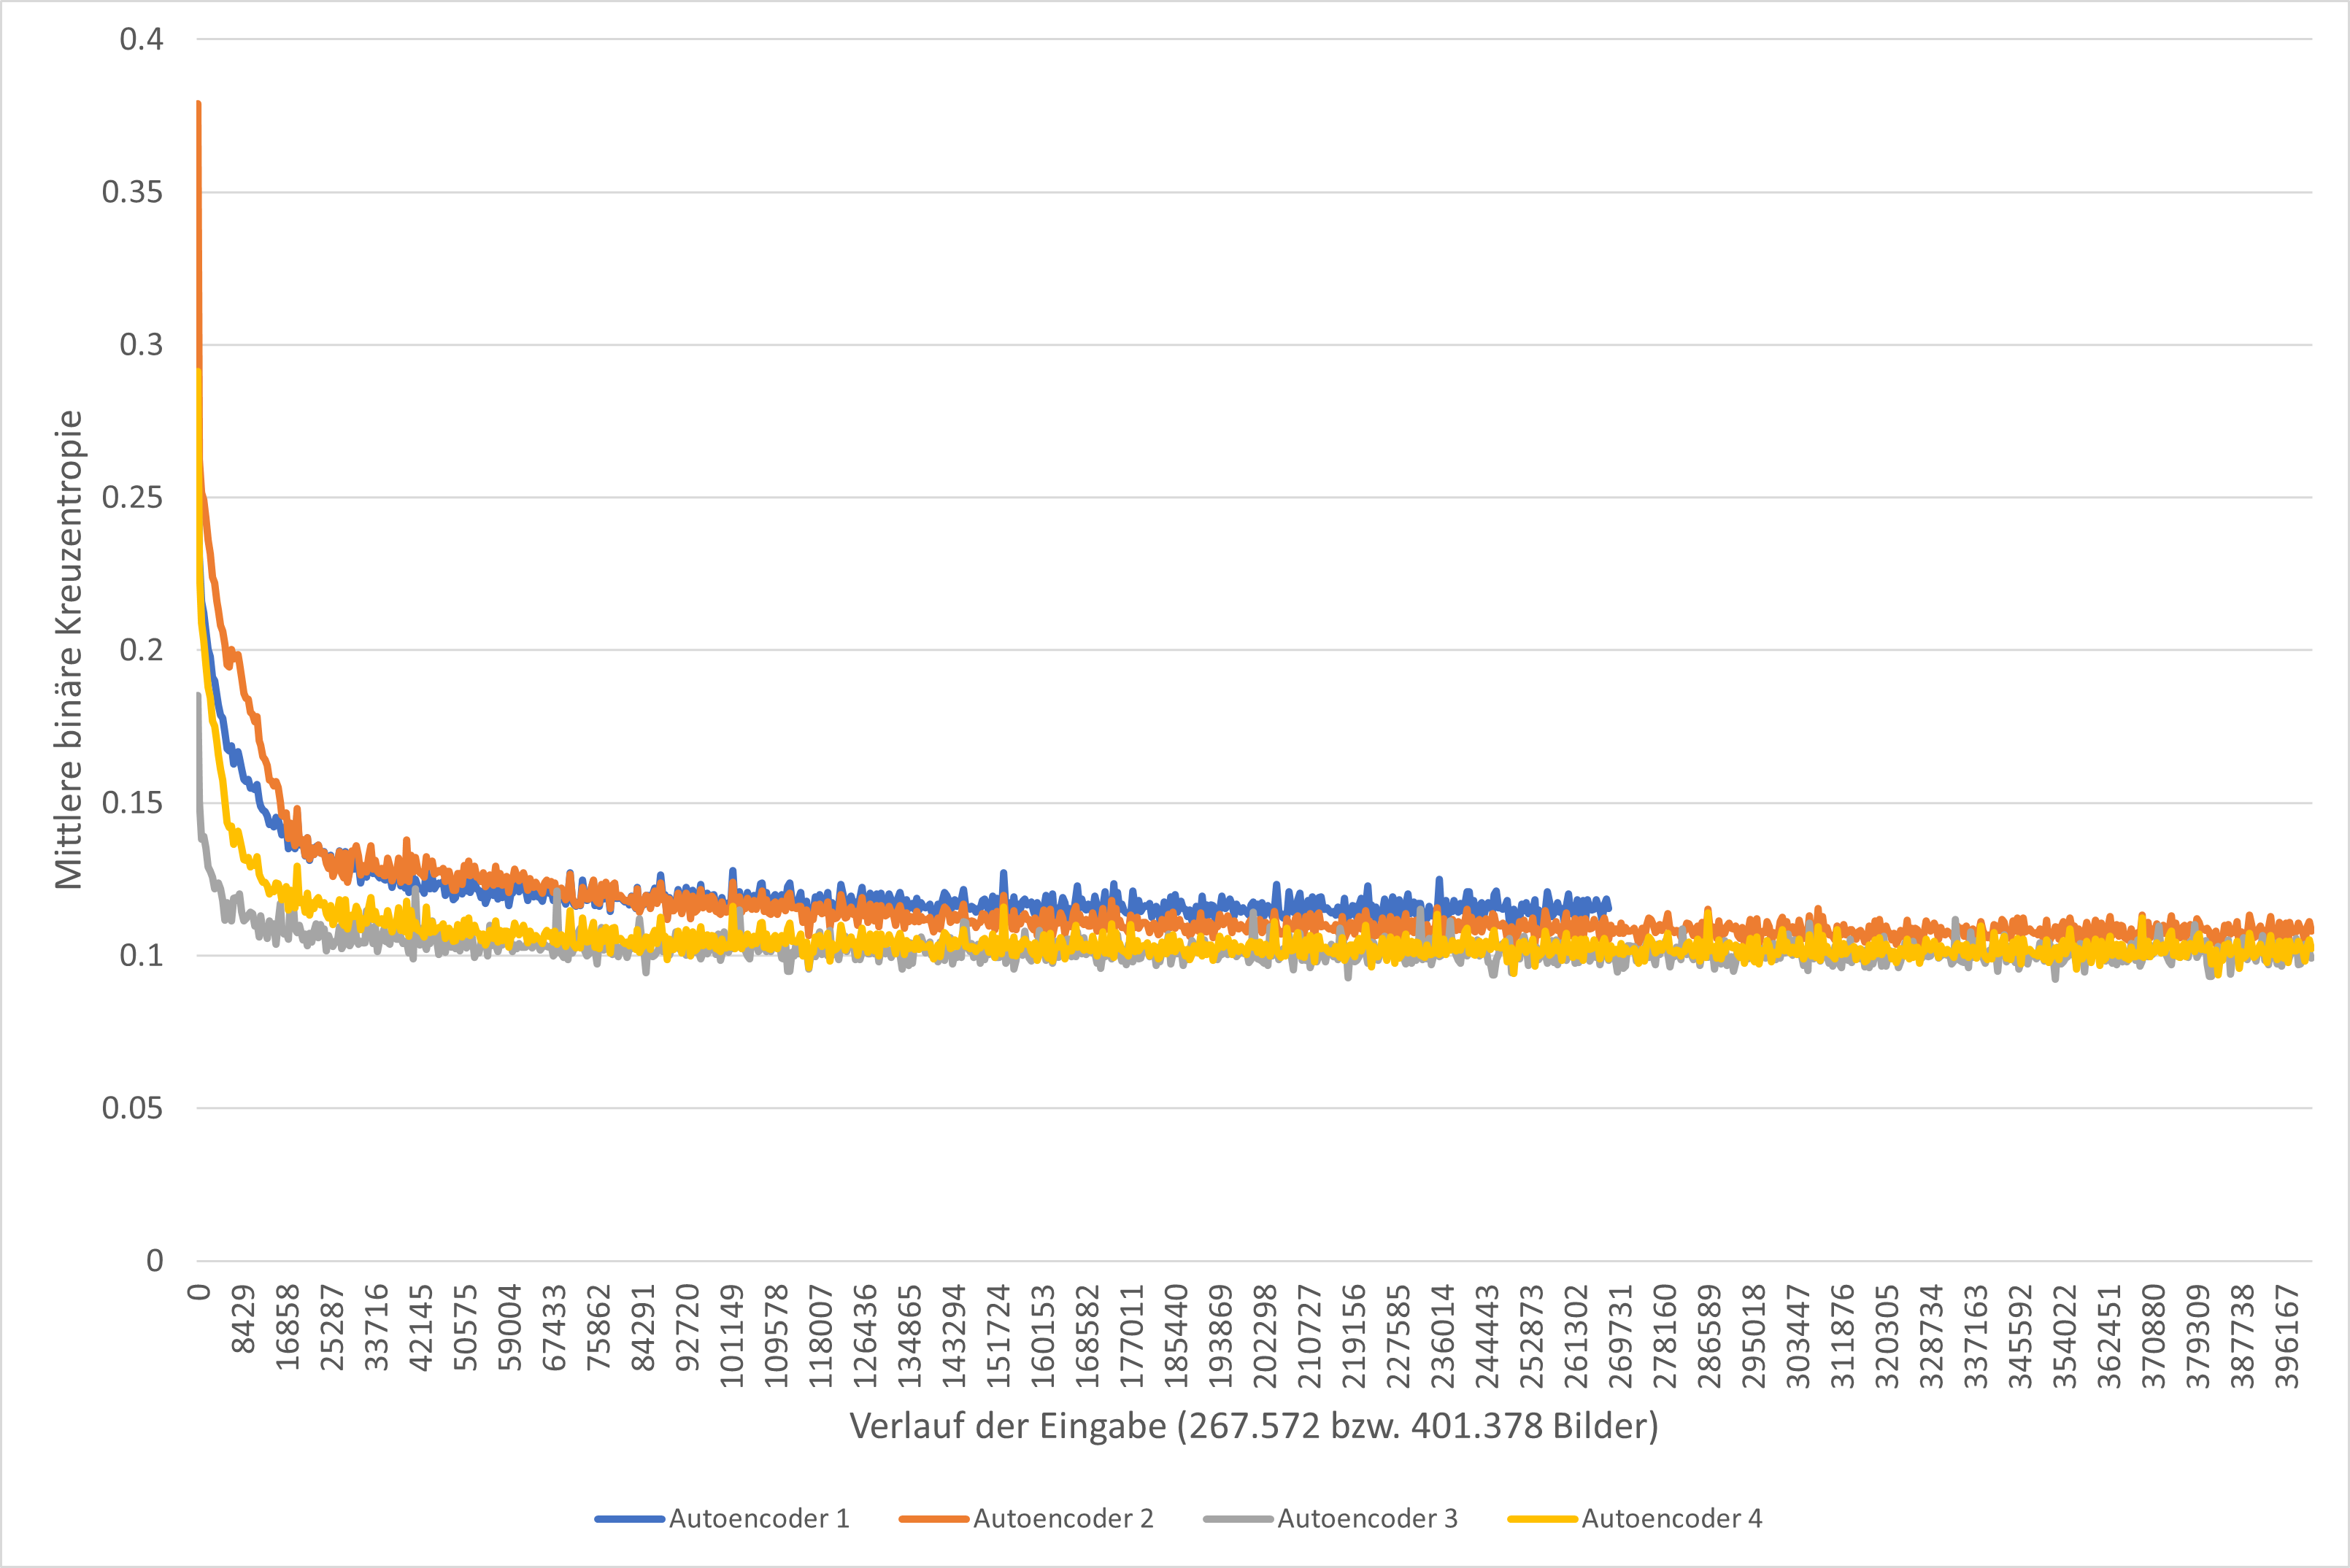
\includegraphics[width=\textwidth]{bilder/training_diagram.png}
            \captionof{figure}{Über 300 bzw. 400 Eingaben gemittelte binäre Kreuzentropie im Lauf des Trainings}
            \label{fig:training_loss}
                \renewcommand{\arraystretch}{1.5}
        \end{minipage}
        }
        \end{center}
\end{figure}


\begin{figure}[htbp]
    \centering
    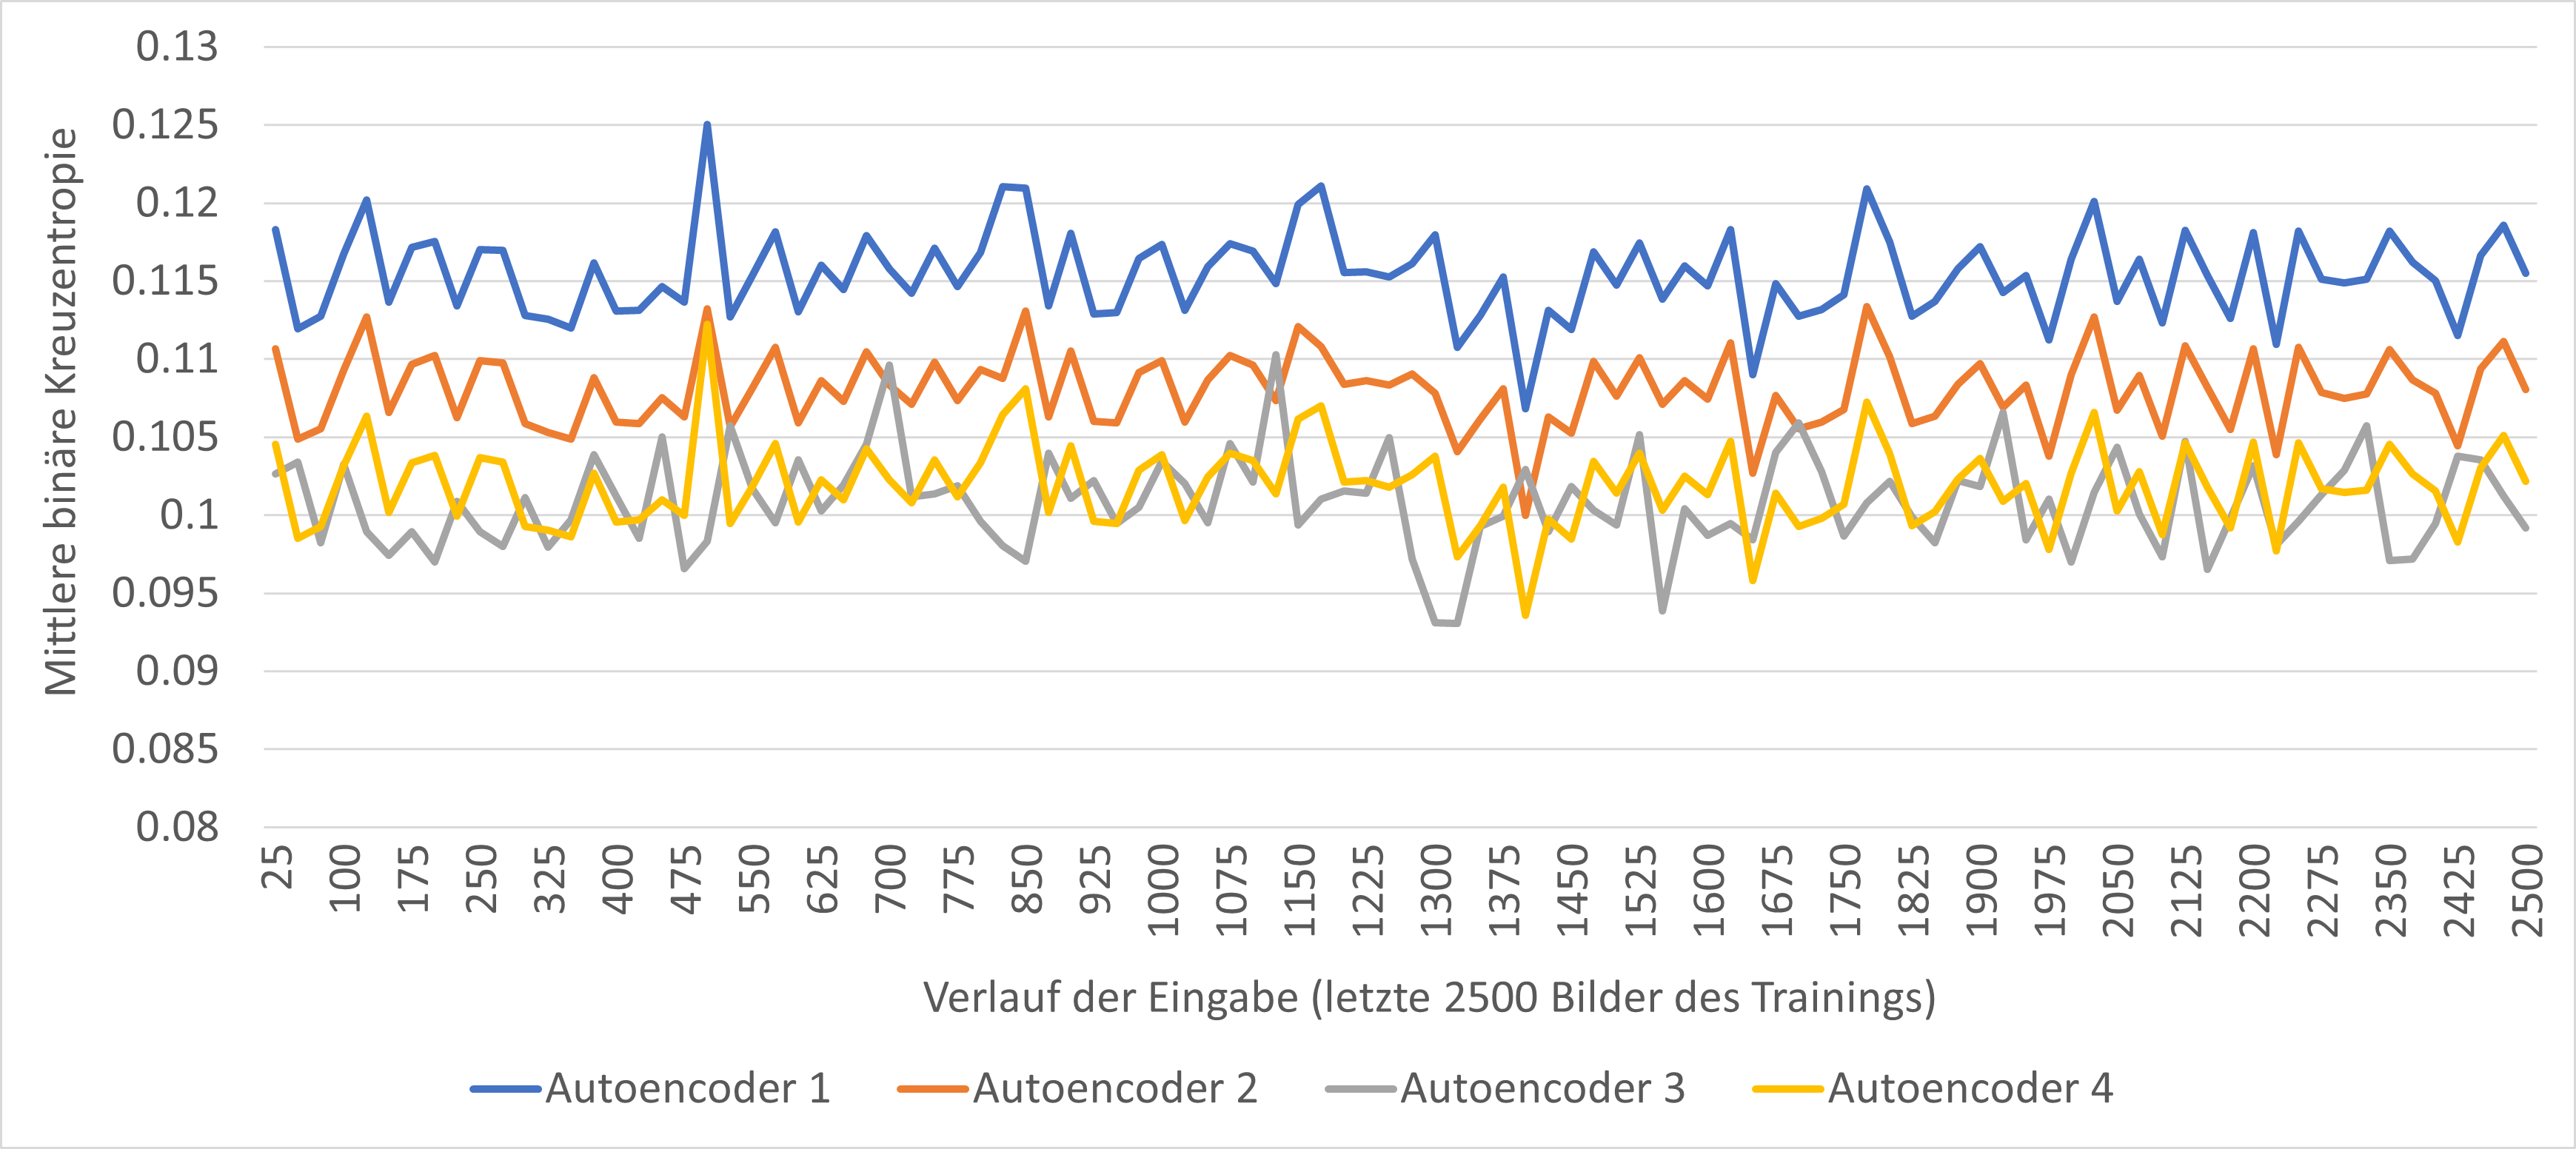
\includegraphics[width=\textwidth]{bilder/training_diagram_last2500.png}
    \caption{Über 300 bzw. 400 Eingaben gemittelte binäre Kreuzentropie der 2500 letzten Batches jedes Autoencoders während des Trainings}
    \label{fig:training_loss_2500}
\end{figure}

\section{Experimente}
Die Autoencoder wurden nach den oben beschriebenen Kriterien trainiert und auf verschiedene Arten und Weisen untersucht. Hierzu wurden mehrere Experimente durchgeführt, in welchen die Generalisierfähigkeit der Autoencoder auf dem Testdatensatz, gegenüber der realen JADX-Applikation sowie gegenüber anderen \glspl{gui} untersucht wurde.

\subsection{Experiment 1 -- MSE auf Testdatensatz}
\label{subsec:exp1}

Das erste durchgeführte Experiment war eine Messung der Qualität der Rekonstruktionen der verschiedenen Autoencoder auf den Testdaten. Hierzu wurden der komplette Testdatensatz als Eingabe für die Autoencoder verwendet und die Ausgaben generiert. Anschließend wurde die Abweichung zwischen Eingabe und Ausgabe mit dem \gls{mse} berechnet und über alle Bilder gemittelt.

\subsubsection*{Ergebnisse}

Die Ergebnisse der Autoencoder-Architekturen unterscheiden sich dabei deutlich und werden in Tabelle~\ref{tab:exp1results} dargestellt.
Autoencoder~\ref{a3} und \ref{a4} schneiden hier am besten ab, während Autoencoder~\ref{a1} und \ref{a2} vergleichsweise schlechte Werte erzielen. So betragen die Mittelwerte des \gls{mse} mehr als das Doppelte des Wertes des Autoencoders~\ref{a3}.


\begin{table}[htbp]
    \centering
    \caption{Ergebnisse der Autoencoder bei Eingabe des Testdatensatzes }
    \label{tab:exp1results}
    \smallskip
    \begin{tabular}{ llll }
        \toprule
        Architektur & Mittelwert des \gls{mse} \\
        \hline
        Autoencoder 1 & $0,004295$ \\
        Autoencoder 2 & $0,003450$ \\
        Autoencoder 3 & \textbf{0,001643} \\
        Autoencoder 4 & $0,001785$ \\
        \bottomrule
    \end{tabular}
\end{table}


\subsubsection*{Fazit}

Ein Unterschied zwischen der Architektur von Autoencoder~\ref{a1} und den anderen Autoencodern liegt in der Verwendung der ReLU-Aktivierungsfunktion anstatt der LeakyReLU-Funktion. Obwohl Ergebnisse von Hu et al.~\cite{huImprovingConvolutionalNeural2018} indizieren, dass die Verwendung der LeakyReLU bei Convolutional-Networks die Ergebnisse um 1-2\% verbessern können, lässt sich dadurch nicht der deutlich schlechtere \gls{mse} erklären. Einen größeren Einfluss auf den schlechteren \gls{mse} dürfte das mit 60~Neuronen vergleichsweise kleine Bottleneck von Autoencodern~\ref{a1} haben. Daher kann es nicht so viele Informationen speichern wie die Bottlenecks der anderen Autoencoder. Autoencoder~\ref{a2} schneidet trotz des sehr großen Bottlenecks von 320~Neuronen ebenfalls vergleichsweise schlecht ab. Dies ist ein Indiz dafür, dass Fully-Connected-Schichten die Ergebnisse gegenüber der ausschließlichen Verwendung von Convolutional-Schichten verbessern können. Dieser Eindruck wird durch die Ergebnisse von Autoencoder~\ref{a3} und \ref{a4} bestärkt, in welchen der Anteil an Fully-Connected-Schichten deutlich höher als in Autoencoder~\ref{a1} ist. Darüber hinaus ist das Bottleneck deutlich breiter.

\subsection{Experiment 2 -- Qualitativer Vergleich der Ergebnisse auf Testdaten}
\label{subsec:exp2}


\begin{figure}[htbp]
    \centering
    \resizebox*{!}{.98\textheight}{\input{AusgabenExp2_1.pdf_tex}}
    \caption{Experiment 2: Vergleich des Bild 1 mit den Ausgaben der Autoencoder. Hochauflösende Bilder siehe Abschnitt \ref{sec:appendix:exp2}}
    \label{exp2_image:1}
\end{figure}

\begin{figure}[htbp]
    \centering
    \resizebox*{!}{.98\textheight}{\input{AusgabenExp2_2.pdf_tex}}
    \caption{Experiment 2: Vergleich des Bild 2 mit den Ausgaben der Autoencoder. Hochauflösende Bilder siehe Abschnitt \ref{sec:appendix:exp2_2}}
    \label{exp2_image:2}
\end{figure}

In diesem Experiment wurden die trainierten Autoencoder qualitativ untersucht. Für diese Masterarbeit ist insbesondere wichtig, dass eine Rekonstruktion als Applikation gut bedienbar wäre sowie die einzelnen \gls{gui}-Elemente sichtbar sind. Eine rein quantitative Betrachtung des \gls{mse} reicht daher nicht aus. Die qualitative Analyse wurde so durchgeführt, dass alle Autoencoder 32 zufällig aus den Testdatensatz ausgewählte Bilder als Eingabe bekamen. Zur Darstellung in dieser Arbeit wurden davon zwei beispielhafte Bilder ausgewählt, anhand welcher die Ergebnisse sowie die Vor- und Nachteile der verschiedenen Autoencoder erklärt werden. Diese Auswahl erfolgte dabei unter der Prämisse, möglichst viele verschiedene \gls{gui}-Elemente der Anwendung JADX darzustellen, um exemplarisch für den Datensatz stehen zu können. Das erste Bild zeigt die Textsuche von JADX und wird zusammen mit den Ausgaben der Autoencoder und deren \gls{mse} in Abb.~\ref{exp2_image:1} dargestellt. Das zweite Bild und die dazugehörigen Ausgaben der Autoencoder bzw. der \gls{mse} befindet sich in Abb.~\ref{exp2_image:2}.

In Tabelle~\ref{tab:exp2results_mse} werden darüber hinaus der \gls{mse} der Autoencoder-Ausgaben auf dem gesamten Testdatensatz mit dem \gls{mse} der für diesen Abschnitt erstellten Untermenge verglichen. Die Abweichung zwischen dem \gls{mse} des Testdatensatzes und der Untermenge ist jeweils gering und liegt ausschließlich im einstelligen Prozentbereich.

\begin{table}[htbp]
    \centering
    \caption{Mittelwert des MSE der Autoencodern-Ergebnisse bei Eingabe des Testdatensatzes und der Untermenge des Testdatensatzes (32 Bilder)}
    \label{tab:exp2results_mse}
    \smallskip
    \begin{tabular}{ llll }
        \toprule
        Architektur & \gls{mse} Testdatensatz & \gls{mse} Untermenge \\
        \hline
        Autoencoder 1 & $0,004295$ & $0,004139$\\
        Autoencoder 2 & $0,003450$ & $0,003326$\\
        Autoencoder 3 & \textbf{0,001643} & \textbf{0,001746}\\
        Autoencoder 4 & $0,001785$ & $0,001944$\\
        \bottomrule
    \end{tabular}
\end{table}

\subsubsection*{Ergebnisse}
Die in diesem Abschnitt beschriebenen Ergebnisse beziehen sich auf die komplette Untermenge des Datensatzes, bestehend aus 32 Bildern. Alle beschriebenen Effekte werden in den Abb.~\ref{exp2_image:1} und \ref{exp2_image:2} dargestellt und können dort nachvollzogen werden.

In der Ausgabe von Autoencoder~\ref{a1} sind alle \gls{gui}-Elemente erkennbar. Über das ganze Bild verteilt befinden sich kleine blaue aber auch schwarze Artefakte -- eine Art Schleier --, womit die Lesbarkeit der Schrift und die Erkennbarkeit von Buttons erschwert ist. Des Weiteren sind deutlich sichtbare Schachbrettmuster erkennbar. Im zweiten Bild wird ersichtlich, dass die blaue, von Windows stammende Kopfleiste nicht klar vom Hintergrund separiert ist und am rechten Rand häufig unvollständig dargestellt wird. Der Button zum Schließen des Fensters wird damit nicht korrekt dargestellt. Ränder von Buttons sind teilweise verwaschen, so in etwa das Feld zur Auswahl des Editor-Themes im Einstellungsfenster von Bild~2. Weiße Buttons auf grauem Hintergrund (sichtbar am unteren Rand des Einstellungsfensters auf Bild~2) sind nicht klar vom Hintergrund abgegrenzt und damit nicht zwangsläufig als Buttons identifizierbar.

Autoencoder~\ref{a2} gibt ein deutlich von Artefakten freieres Bild aus und zeigt darüber hinaus alle \gls{gui}-Elemente klar erkennbar. Die blaue Kopfleiste wird vollständig angezeigt und beinhaltet nur kleine Artefakte. Das Schriftbild ist im Vergleich zu Autoencoder~\ref{a1} zwar freier von Artefakten, dennoch etwas unscharf. Im Vergleich zu Autoencoder~\ref{a1} ist der Kontrast geringer, wodurch das Bild homogener wirkt. Manche Linien erscheinen dennoch nur in einem hellen statt kräftigen Grauton.

Das Ergebnis von Autoencoder~\ref{a3} ist schärfer und kontrastreicher, wodurch das Schriftbild klarer wird. Farbtöne sind insgesamt kräftiger als bei Autoencoder~\ref{a2}, ohne die starken Artefakte von Autoencoder~\ref{a1}. Insbesondere Ränder von Buttons und sonstigen \gls{gui}-Elementen sind vergleichsweise scharf dargestellt. Die blaue Kopfleiste ist sehr trennscharf und einheitlich vom Hintergrund separiert und wird komplett dargestellt. Weiße Buttons auf grauem Hintergrund sind im Vergleich zu Autoencoder~\ref{a1} besser abgegrenzt, jedoch durch die unscharfe Umrandung nicht direkt als Button identifizierbar.

Die Ergebnisse des Autoencoders~4 sind in etwa auf dem Niveau des Autoencoders~3. Im Vergleich sind die Bilder weniger kontrastreich, dafür werden jedoch Flächen etwas gleichmäßiger dargestellt.

Wenn man den \gls{mse} betrachtet, so werden die Ergebnisse aus Experiment~1 aus Abschnitt~\ref{subsec:exp1} hier bestätigt. Autoencoder~\ref{a3} und \ref{a4} schneiden am besten ab, gefolgt von Autoencoder~\ref{a2} und zuletzt Autoencoder~\ref{a1}. Die Werte liegen dabei sehr nah an den Durchschnittswerten aus Experiment 1. Lediglich die Ausgabe von Autoencoder~\ref{a2} weist etwas bessere Werte auf.

\subsubsection*{Fazit}
Autoencoder~\ref{a3} und \ref{a4} schneiden hier am besten ab, da die Bildqualität auf der untersuchten Untermenge des Testdatensatzes besser ist, als bei Autoencoder~\ref{a1} und \ref{a2}. Darüber hinaus liegt der \gls{mse} bei diesen deutlich niedriger. Autoencoder~\ref{a3} und \ref{a4} sind dabei auf ähnlichem Niveau, wobei Autoencoder~\ref{a3} kontrastreichere Bilder ausgibt und Autoencoder~\ref{a4} Flächen etwas homogener darstellt. Der \gls{mse} ist bei Autoencoder~\ref{a3} am geringsten. Autoencoder~\ref{a1} fällt gegenüber den anderen Autoencodern durch die schlechtere Bildqualität und die deutlich sichtbaren Schachbrettmuster ab.

\subsection{Experiment 3 -- Verwendung von Daten der Anwendung JADX}
\label{subsec:exp3}
Ein wichtiger Aspekt in der Bewertung von Autoencoder-Architekturen ist die Fähigkeit zur Generalisierung. In diesem Kontext bedeutet dies nicht nur, den Fehler auf Trainings- und Testdaten zu minimieren, sondern auch auf Daten der realen Applikation. Die Autoencoder sollen letztendlich mit echten \gls{gui}-Daten arbeiten. Daher ist es wichtig zu analysieren, wie gut sie auf echten Daten funktionieren. Insbesondere ist hier wichtig, wie schwer die in Abschnitt~\ref{sec:mock_limitations} besprochenen Unterschiede zwischen Mock und realer \gls{gui} wiegen.

\begin{figure}[htbp]
    \centering
    \resizebox*{!}{.98\textheight}{\input{AusgabenExp3_1.pdf_tex}}
    \caption{Experiment 3: Vergleich des Bild 1 mit den Ausgaben der Autoencoder. Hochauflösende Bilder siehe Abschnitt \ref{sec:appendix:exp3}}
    \label{exp3_image:1}
\end{figure}

\begin{figure}[htbp]
    \centering
    \resizebox*{!}{.98\textheight}{\input{AusgabenExp3_2.pdf_tex}}
    \caption{Experiment 3: Vergleich des Bild 2 mit den Ausgaben der Autoencoder. Hochauflösende Bilder siehe Abschnitt \ref{sec:appendix:exp3_2}}
    \label{exp3_image:2}
\end{figure}


Um diese Fragestellungen zu untersuchen, wurden 22 Abbilder von JADX untersucht. Von diesen werden hier zwei Bilder zusammen mit den Ausgaben der Autoencoder dargestellt. Die 22 Abbilder wurden so ausgewählt, dass sie möglichst viele Facetten von JADX zeigen sollen. Darin enthalten sind sowohl Elemente, die im Mock abgebildet werden, wie die Hauptansicht oder die Textsuche, aber auch Elemente, die nur in der realen JADX-Applikation existieren. Dazu gehören bspw. die Dialoge, um Daten zu öffnen, oder das JADX-Log anzuzeigen. Genaueres zu den Unterschieden der Hauptansicht wird in Abschnitt~\ref{sec:mock_limitations} erklärt. Das erste, hier dargestellte Bild enthält die Hauptansicht von JADX. Die meisten Elemente dieser Ansicht wurden so direkt im Mock, auf welchem die Autoencoder trainiert wurden, abgebildet. Dennoch existieren hier auch Unterschiede, wie die Speicherverbrauchsanzeige am unteren Bildrand, die nicht im Mock implementiert ist. Diese ist daher nicht in den Trainingsdaten vorhanden und stellt für die Autoencoder ein komplett neues Element dar.

Das zweite Bild beinhaltet eine Ansicht, die im entwickelten Mock der \gls{gui} so nicht existiert: das Fenster um Dateien zu öffnen. Dieses wird nur unter Windows so dargestellt, wie abgebildet. Es orientiert sich an der Windows zugrundeliegenden Designsprache. Deshalb ist es der Designsprache von JADX unter Windows, und damit des Mocks, ähnlich.

Die Bilder wurden als Eingabe für jeden Autoencoder verwendet und analysiert. Dabei wurde jeweils der \gls{mse} berechnet und die Bilder einer qualitativen Analyse unterzogen. Die zwei ausgewählten Eingabebilder und die Ergebnisse der Autoencoder zusammen mit dem berechneten \gls{mse} werden in Abb.~\ref{exp3_image:1} und \ref{exp3_image:2} dargestellt.
Ein Vergleich des \gls{mse} des kompletten Datensatzes mit dem \gls{mse} des Testdatensatzes befindet sich in Tab.~\ref{tab:exp3results_mse}.

\begin{table}[htbp]
    \centering
    \caption{Mittelwert des MSE der Autoencoder-Ausgaben bei Eingabe des Testdatensatzes und der Bilder der JADX-Applikation (22 Bilder)}
    \label{tab:exp3results_mse}
    \smallskip
    \begin{tabular}{ llll }
        \toprule
        Architektur & \gls{mse} Testdatensatz & \gls{mse} Datensatz JADX \\
        \hline
        Autoencoder 1 & $0,004295$ & $0,011156$\\
        Autoencoder 2 & $0,003450$ & $0,010440$\\
        Autoencoder 3 & \textbf{0,001643} & $0,009843$\\
        Autoencoder 4 & $0,001785$ & \textbf{0,009283}\\
        \bottomrule
    \end{tabular}
\end{table}

\pagebreak
\subsubsection*{Ergebnisse}
Die Resultate des 2. Experimentes aus Abschnitt \ref{subsec:exp2} lassen sich weitgehend auf alle hier untersuchten Bilder übertragen. Insbesondere die im vorigen Experiment aufgetretenen Artefakte bei Autoencoder~\ref{a1}, die leichte Unschärfe und Kontrastarmut bei Autoencoder~\ref{a2} und die bessere Darstellung von Flächen durch Autoencoder~\ref{a4} sind auch hier auffällig.

Im Besonderen wird die Hauptansicht (sichtbar in Abb.~\ref{exp3_image:1}) von allen Autoencodern so rekonstruiert, dass der Projektbaum in der linken Bildhälfte und der Editor in der rechten Bildhälfte erkennbar bleiben. Größere Unterschiede treten bei den Elementen auf, die nicht im Mock vorkommen. Die grüne Leiste als Teil der Speicherverbrauchsanzeige wird bei Autoencoder~\ref{a1} nur extrem schwach oder gar nicht angezeigt. Die textuelle Repräsentation des Speicherverbrauchs ist zwar in Andeutungen erkennbar, aber unlesbar. Autoencoder~\ref{a2} zeigt zwar die Leiste der Speicherverbrauchsanzeige an, wenn auch teilweise in einer verfälschten Farbe. Der Text ist jedoch ebenfalls größtenteils unlesbar. Autoencoder~\ref{a3} und \ref{a4} können die Leiste zwar darstellen, allerdings ist diese bei den Ausgaben beider Autoencoder auf den meisten Bildern des Datensatzes unvollständig. Bei Autoencoder~\ref{a4} wird die Farbe der Leiste korrekt wiedergegeben. Der dazugehörige Text ist sowohl bei Autoencoder~\ref{a3} als auch bei Autoencoder~\ref{a4} unscharf, aber lesbar.

Ein weiteres, nur in der realen JADX-Applikation vorkommendes Element ist die über der Speicherverbrauchsanzeige liegende Tab-Navigation. Mit dieser kann zwischen Java-Code und der Smali-Notation (einer Art Java-VM-Assembler) gewechselt werden. Diese wird von den Autoencodern~\ref{a3} und \ref{a4} am besten dargestellt. Hier ist sowohl erkennbar, dass es sich um Buttons handelt, als auch, welcher Tab ausgewählt ist. Die übrigen Autoencoder stellen zwar den Text dar, die Buttons sind jedoch nicht oder nur schlecht als solche identifizierbar. Die Balken rund um den Editor und den Projektbaum, über die eine Scrollfunktion implementiert ist, werden von Autoencoder~\ref{a3} und \ref{a4} dargestellt. Autoencoder~\ref{a1} stellt lediglich einen der Balken korrekt dar, während in den Ausgaben des Autoencoders~\ref{a2} kein Balken sichtbar ist.

Neben den Elementen, die nicht im Mock vorkommen, gibt es auch bei der Darstellung des Menüs und der Icon-Leiste am oberen Bildrand Unterschiede zwischen den einzelnen Autoencodern. Lediglich Autoencoder~\ref{a4} stellt beides in einer solchen Qualität dar, dass alle Elemente erkennbar sind. Bei den Autoencodern~\ref{a1} und \ref{a2} sind sowohl der Text als auch die Icons teilweise nur schwach sichtbar. Autoencoder~\ref{a3} gibt den Text und die Icons stärker aus. Über dem linken oberen Eck des Bildes liegt jedoch bei einigen Bildern (erkennbar in Abb.~\ref{exp3_image:1}) eine Art großflächige Störung vor, welche den Text und die Icons teilweise unlesbar macht. Diese tritt vor allem bei Auswahl des Hauptfensters von JADX auf, wodurch sich die Windows-Kopfleiste blau färbt. Lediglich die Ergebnisse von Autoencoder~\ref{a4} sind so geartet, dass der Text lesbar ist und die Mehrzahl der Icons gut identifizierbar bleibt.

Zusätzliche Fenster, bspw. das in Abb.~\ref{exp3_image:2} dargestellte Fenster zum Öffnen einer Datei, werden von allen Autoencodern so dargestellt, dass der Inhalt lesbar und die Icons identifizierbar sind. Die Darstellungsqualität der einzelnen Elemente schwankt jedoch deutlich, sodass Autoencoder~\ref{a1} die bekannten Artefakte insbesondere bei Flächen und Icons aufweist und Autoencoder~\ref{a2} die Schrift und die Icons eher schwach darstellt. Die Ausgabe der Autoencoder~\ref{a3} und \ref{a4} enthält die Elemente in besserer Darstellungsqualität, wobei die Icons kontrastarm angezeigt werden. Insbesondere Ränder um Buttons und Eingabefelder werden hier scharf dargestellt. Eingefärbte Flächen, bspw. gelb-markierte Code-Bereiche wie in Abb.~\ref{exp3_image:1}, werden von Autoencoder~\ref{a3} und \ref{a4} teilweise blau anstatt in der Ursprungsfarbe eingefärbt. Eine Erklärungsmöglichkeit hierfür liegt darin, dass Autoencoder diese Bereiche womöglich als blaue Windows-Kopfleiste einstufen, weshalb eine Farbverwechslung erfolgt.

Wenn man den \gls{mse} betrachtet, so werden die großen Abstände in den Ergebnissen aus Experiment~1 des Abschnittes~\ref{subsec:exp1} hier deutlich kleiner. Auffällig ist, dass Autoencoder~\ref{a4} in diesem Experiment einen niedrigeren \gls{mse} erreicht als Autoencoder~\ref{a3}. Autoencoder~\ref{a4} erreicht nach dem \gls{mse} bei 18 von 22 Bildern ein besseres Ergebnis als Autoencoder~\ref{a3}. Dieser Abstand wird bei den Bildern, in welchen bei Autoencoder~\ref{a3} die Störung aus Bild~1 auftritt, deutlicher. Der Wert von Autoencoder~\ref{a3} liegt dort näher bei den Werten der Autoencoder~\ref{a1} und \ref{a2}.


\subsubsection*{Fazit}
Autoencoder~\ref{a4} schneidet in diesem Experiment sowohl bzgl. des \gls{mse} als auch in der qualitativen Analyse am besten ab, da er das Originalbild am besten rekonstruieren kann. Bei einigen Bildern, wie Bild 1, liegt der Wert des Autoencoders~\ref{a4} deutlich vor den weiteren Autoencodern, während bei Bild~2 Autoencoder~\ref{a3} und \ref{a4} auf einem ähnlichen Niveau abschneiden.

Die Frage nach den besten Fähigkeiten zur Generalisierung kann -- jedenfalls im Rahmen dieses Experiments -- Autoencoder~\ref{a4} für sich entscheiden. Dieser konnte am besten mit den Unterschieden zwischen dem Mock und JADX umgehen. Die Elemente, die nicht im Mock enthalten sind, werden von Autoencoder~\ref{a4} am genauesten dargestellt. Bei diesem Autoencoder treten auch die wenigsten Bildstörungen auf.

\subsection{Experiment 4 -- Verwendung von weiteren GUIs}
\label{subsec:exp4}

Der nächste Schritt in der Generalisierung besteht darin, \glspl{gui} als Eingabe für die Autoencoder zu verwenden, auf denen kein Training stattfand. Die zugrundeliegende Fragestellung ist die, ob ein Autoencoder so entwickelt werden kann, dass er für ganze Familien von Anwendungen geeignet ist. Um diese Fragestellungen stichprobenhaft zu untersuchen, wurden zwei Abbilder von Anwendungen als Eingabe für die Autoencoder verwendet. Das erste Bild zeigt den Windows Explorer. Dieser wurde ausgewählt, da er eine vollständig unterschiedliche Anwendung darstellt, im Kern jedoch einer ähnlichen Designsprache folgt. Der Windows Explorer ist strukturell ähnlich zu JADX aufgebaut: Einem zweispaltiges Layout bestehend aus einer Baumstruktur in der linken Spalte sowie zeilenweisen Einträgen in der rechten Spalte. Das Farbschema ist dem von JADX ähnlich und besteht hauptsächlich aus Weiß- und Grautönen sowie dem Blauton der Windows-Kopfleiste. Darüber hinaus ist der Inhalt -- genau wie bei JADX -- sehr textlastig und wird durch die häufige Verwendung kleiner Icons unterstützt.

Das zweite, verwendete Bild ist ein Screenshot der Webseite des Repositories dieser Masterarbeit auf GitHub\footnote{\url{https://github.com/research-manuscripts/MA_Felix_Rittler}, letzter Zugriff: 13.11.2021} (Stand: 13.11.2021). Im Vergleich zu JADX und dem Windows Explorer kommt hier eine völlig andere Designsprache zum Einsatz. Erstens ist der \emph{Dark Mode} von GitHub aktiviert, sodass das Bild durch einen höheren Anteil sehr dunkler Bereiche geprägt ist. Darüber hinaus unterscheiden sich verwendeten Farben deutlich.

Beide Bilder wurden, wie im vorigen Experiment, als Eingabe für die Autoencoder verwendet. Die Ausgaben und der dazugehörige \gls{mse} werden in Abb.~\ref{exp4_image:1} und \ref{exp4_image:2} dargestellt.

\begin{figure}[htbp]
    \centering
    \resizebox*{!}{.98\textheight}{\input{AusgabenExp3_3.pdf_tex}}
    \caption{Experiment 4: Vergleich des Bild 1 mit den Ausgaben der Autoencoder. Hochauflösende Bilder siehe Abschnitt \ref{sec:appendix:exp4}}
    \label{exp4_image:1}
\end{figure}

\begin{figure}[htbp]
    \centering
    \resizebox*{!}{.98\textheight}{\input{AusgabenExp3_4.pdf_tex}}
    \caption{Experiment 4: Vergleich des Bild 2 mit den Ausgaben der Autoencoder. Hochauflösende Bilder siehe Abschnitt \ref{sec:appendix:exp4_2}}
    \label{exp4_image:2}
\end{figure}

\subsubsection*{Ergebnisse}
Autoencoder~\ref{a3} und \ref{a4} können das Bild des Windows Explorers in besserer Qualität anzeigen als Autoencoder~\ref{a1} und \ref{a2}. Die Defizite bzgl. Störungen und der Darstellung der blauen Kopfleiste treten hier wie in Experiment~3 in Abschnitt~\ref{subsec:exp3} auf. Autoencoder~\ref{a2} verursacht diese zwar nicht, gibt das Bild aber insgesamt kontrastarm wieder. Einige Icons, aber auch Text, werden sehr hell dargestellt, wodurch die Erkennbarkeit und Lesbarkeit erschwert werden. Bei Autoencoder~\ref{a3} ist die Lesbarkeit deutlich besser, jedoch tritt hier wieder die aus Experiment~\ref{subsec:exp3} bekannte Bildstörung in der oberen linken Bildecke auf. Autoencoder~\ref{a4} schafft es, alle Bildelemente am besten darzustellen. Der Kontrast ist vor allem gegenüber Autoencoder~\ref{a2} -- aber bei Icons auch gegenüber Autoencoder \ref{a3} -- höher, ohne, dass dabei Bildstörungen entstehen. Der Text ist bei der Ausgabe von Autoencoder~\ref{a4} sehr gut lesbar, wobei ihm dies am unteren Bildrand besser gelingt als Autoencoder~\ref{a3}.

Der gemessene \gls{mse} bestätigt die Ergebnisse. Während Autoencoder~\ref{a2} bis \ref{a3} auf ähnlichem Niveau im Bereich zwischen $0,0074$ und $0,0078$ liegen, liegt Autoencoder~\ref{a4} mit $0,0058$ deutlich darunter. Autoencoder~\ref{a1} weist mit $0,0085$ eindeutig den schlechtesten Wert auf.

Das Bild der Webseite wird von allen Autoencodern stark verfälscht rekonstruiert. Kein Autoencoder stellt die Farbe der Webseite dar, lediglich bei Autoencoder~\ref{a1} sind immerhin Teile in einer verfälschten Farbe eingefärbt. Der Text ist nur bei Autoencoder~\ref{a2} in Ansätzen erkennbar. Autoencoder~\ref{a3} und \ref{a4} stellen lediglich die Flächen, auf denen sich im Originalbild Inhalt befindet, korrekt dar. Der Inhalt ist jedoch nicht les- oder erkennbar. Betrachtet man die zum Webbrowser gehörenden \gls{gui}-Elemente, verändert sich das Bild etwas. Hier schneiden wie bei allen Bildern zuvor Autoencoder~\ref{a3} und \ref{a4} am besten ab. So stellen diese die Icons gut erkennbar dar. Auch Autoencoder~\ref{a2} zeigt die Icons, wobei die Unschärfe zunimmt. Die Flächen werden durch Autoencoder~\ref{a2} und \ref{a4} am besten dargestellt. Das von Autoencoder~\ref{a1} ausgegebene Bild weist die bereits beobachteten Artefakte auf und zeigt einige Icons nur sehr schwach. Die Lesbarkeit der Schrift ist an dieser Stelle ebenso nicht gegeben.
Der gemessene \gls{mse} ist bei allen Autoencodern sehr hoch und ist nahe bei $0,5$. Diesbezüglich schneidet kein Autoencoder deutlich besser oder schlechter ab.

\subsubsection*{Fazit}
Die Ausgaben der Autoencoder zu Bild~1 sind in ihrer Qualität vergleichbar zu den Ergebnissen, die diese bei Eingabe der realen JADX Applikation in Experiment~3 erreichen. Dies wird durch den gemessenen \gls{mse} untermauert, bei dem alle Autoencoder bei Bild~1 sogar besser abschneiden, als bei Bild~1 aus Experiment~2. Es ist auch hier so, dass Autoencoder~\ref{a4} die besten Ergebnisse erzielt.
Der Wert von Autoencoder~\ref{a3} wird besonders von dem gestörten Bildbereich negativ beeinflusst.

Die Ergebnisse ändern sich bei Bild~2 jedoch deutlich. Kein Autoencoder schafft es, die Webseite in akzeptabler Qualität darzustellen. Eine Erklärungsmöglichkeit ist in dem vollständig anderen Farbschema der Webseite zu finden. Alle anderen Eingaben für die Autoencoder (Testdaten, JADX und der Windows Explorer) sind in ihrer Designsprache vergleichsweise ähnlich und bestehen überwiegend aus hellen Flächen mit kleinen Icons und schwarzem Text. Die Webseite ist jedoch sehr dunkel. Für diesen Erklärungsansatz spricht, dass die Kopfleiste des Webbrowsers deutlich besser dargestellt wird und deren Rekonstruktion qualitativ näher an den Rekonstruktionen der Autoencoder aus den anderen Experimenten ist.

Auch wenn die Ergebnisse dieses Experiments durch die Datenmenge in Gestalt einer kleinen Stichprobe nur eine eingeschränkte Aussagekraft haben, lassen sich hier die Grenzen der Autoencoder aufzeigen. So kann man zum einen ableiten, dass sich prinzipiell auch auf anderen Applikationen als jener, mit der das Training stattfand, gute Ergebnisse erzielen lassen. Die Rekonstruktion der Ansichten unter Verwendung komplett unterschiedlicher Farbschemata ist jedoch komplexer und mit den hier entwickelten Autoencodern und den derzeitigen Trainingsdaten nicht möglich.

\subsection{Experiment 5 -- Geschwindigkeit}
\label{subsec:exp5}
Nicht zuletzt ist auch die Geschwindigkeit der Autoencoder ein wichtiger Parameter, um diese zu bewerten. Im Zusammenhang mit neuronalen Netzen wird in der Regel die Inferenzzeit zur Bewertung verwendet. Die Inferenzzeit bezeichnet die benötigte Zeit, um aus einer Eingabe eine Vorhersage zu berechnen. Nicht Teil dieser Zeit sind insbesondere die Vorgänge, um Daten auf die \gls{gpu} zu verschieben, zur Initialisierung der Netze und Parameter und der Aufwärmvorgang der \gls{gpu}. Die Inferenzzeit wurde für alle Autoencoder sowohl unter Verwendung der \gls{gpu} als auch der \gls{cpu} berechnet.

Als Host-Rechner wurde eine Workstation des \gls{fzi} verwendet, deren Spezifikationen in Tab.~\ref{tab:workstation} dargestellt werden. Das Modul \texttt{torch.distributed}, das es ermöglicht, mehrere \glspl{cpu} einzubeziehen, blieb bei der Messung der Inferenzzeit außen vor. Daher fanden die Berechnungen immer nur auf einer \gls{cpu} statt.

In diesem Experiment wurde ein zufälliger Eingabevektor 300 mal als Eingabe verwendet und die Inferenzzeiten, wie im vorigen Abschnitt beschrieben, gemessen. Aus den gemessenen 300 Inferenzzeiten wurde der Mittelwert und die Standardabweichung berechnet. Diese Messungen und Berechnungen wurden dabei für jeden der 4 Autoencoder jeweils auf der \gls{cpu} und auf der \gls{gpu} durchgeführt.

\pagebreak
Zusätzlich zu Mittelwert und Standardabweichung wird jeweils noch ein sog. \gls{gpu}-Beschleunigungsfaktor $s$ angegeben.
Dieser beschreibt die mittlere Beschleunigung durch Verwendung der \gls{gpu} statt der \gls{cpu} und wird wie folgt aus dem Mittelwert der Inferenzzeiten auf der \gls{cpu} $\overline{x}_{CPU}$ und dem Mittelwert der Inferenzzeiten auf der \gls{gpu} $\overline{x}_{GPU}$ berechnet:

\begin{equation}
    s = \frac{\overline{x}_{CPU}}{\overline{x}_{GPU}}
\end{equation}

\begin{table}[t]
    \centering
    \caption{Spezifikationen der verwendeten Workstation}
    \label{tab:workstation}
    \smallskip
    \begin{tabularx}{8.3cm}{ lX }
        \toprule
        Komponente & Modell \\
        \hline
        CPU & 2 x Intel Xeon Gold 6258R \\
        CPU-Architektur & Intel Cascade Lake \\
        CPU-Kerne & jew. 28 Kerne à 2,7 GHz mit max. 56 Threads \\
        GPU & Nvidia Tesla V100S 32 GB \\
        Grafikchip & Nvidia Volta GV100 \\
        Arbeitsspeicher & 256 GB \\
        \bottomrule
    \end{tabularx}
\end{table}

\subsubsection*{Ergebnisse und Fazit}
Die Ergebnisse der Messungen und der \gls{gpu}-Beschleunigungsfaktor werden in Tab.~\ref{tab:exp5results} dargestellt. Autoencoder~\ref{a2} erzielt dabei in allen Kategorien die besten Ergebnisse. Dieser gibt sowohl auf der \gls{cpu} als auch auf der \gls{gpu} am schnellsten ein Ergebnis aus. Daneben ist bei diesem Autoencoder der Vorteil bei der Verwendung der \gls{gpu} mit einem Faktor von $55,93$ am höchsten. Autoencoder~\ref{a3} und \ref{a4} erreichen fast identische Werte mit leichten Vorteilen für Autoencoder~\ref{a4}, wohingegen Autoencoder~\ref{a1} vergleichsweise langsam ist. Letzterer besitzt zusätzlich eine deutlich geringere Beschleunigung bei Verwendung der \gls{gpu}.

Über alle Autoencoder hinweg stehen die Inferenzzeiten in Korrelation zur Größe der ersten Convolutional-Schicht. Die vergleichsweise hohe Inferenzzeit des Autoencoders~\ref{a1} lässt sich durch die aufwendigen Berechnungen in der ersten Schicht mit einem 32x32-Filter erklären. Autoencoder~\ref{a2} weißt mit Abstand die geringste Inferenzzeit auf -- eine Tatsache, die sich durch die geringe Filtergröße der ersten Convolutional-Schicht, aber auch durch die fehlenden Fully-Connected-Schichten, erklären lässt. Insbesondere Autoencoder~\ref{a3} und \ref{a4} weisen besonders große Fully-Connected-Schichten auf.

\begin{table}[htbp]
    \centering
    \caption{Mittelwert und Standardabweichung der Inferenzzeit bei Verwendung der CPU bzw. GPU der Workstation und GPU-Beschleunigungsfaktor}
    \label{tab:exp5results}
    \smallskip
    \begin{tabular}{ llllll }
        \toprule
        \multirow{2}{*}{Architektur} & \multicolumn{2}{c}{CPU} & \multicolumn{2}{c}{GPU} & GPU- \\
        \cline{2-5}
        & Mittelwert & Std & Mittelwert & Std & Beschleunigung $s$ \\
        \hline
        Autoencoder 1 & $4,1731s$ & $0,1219$ & $0,2830s$ & $0,0053949$ & $14,75$\\
        Autoencoder 2 & \textbf{0,6779s} & 0,0147 & \textbf{0,0121s} & $0,0005165$ & \textbf{55,93}\\
        Autoencoder 3 & $1,5976s$ & $0,0427$ & $0,0404s$ & $0,0003145$ & $39,58$\\
        Autoencoder 4 & $1,5061s$ & $0,0325$ & $0,0389s$ & $0,0003203$ & $38,67$\\
        \bottomrule
    \end{tabular}
\end{table}

\section{Erfahrungen und Fehlschläge}
Neben den hier vorgestellten Autoencodern~\ref{a1} bis \ref{a4} mit guten Ergebnisse, wurden auch Architekturen entwickelt, die keine guten oder teilweise auch sehr schlechte Ergebnisse erzielten. Diese Ansätze, welche im Rahmen dieser Masterarbeit nicht funktionierten, sollen in diesem Abschnitt dargestellt werden. Es wird hier die Zielsetzung verfolgt, zukünftigen Entwicklern und Forschern weitere Erfahrungen und Anhaltspunkte auf den Weg zu geben. Mit diesen Erfahrungen soll es einfacher werden, bessere Autoencoder zu entwickeln, ohne die gleichen Fehler erneut zu begehen. In diesem Abschnitt werden daher zudem Vermutungen angestellt, warum diese Ansätze nicht funktionierten.

\begin{figure}[htbp]
    \centering
    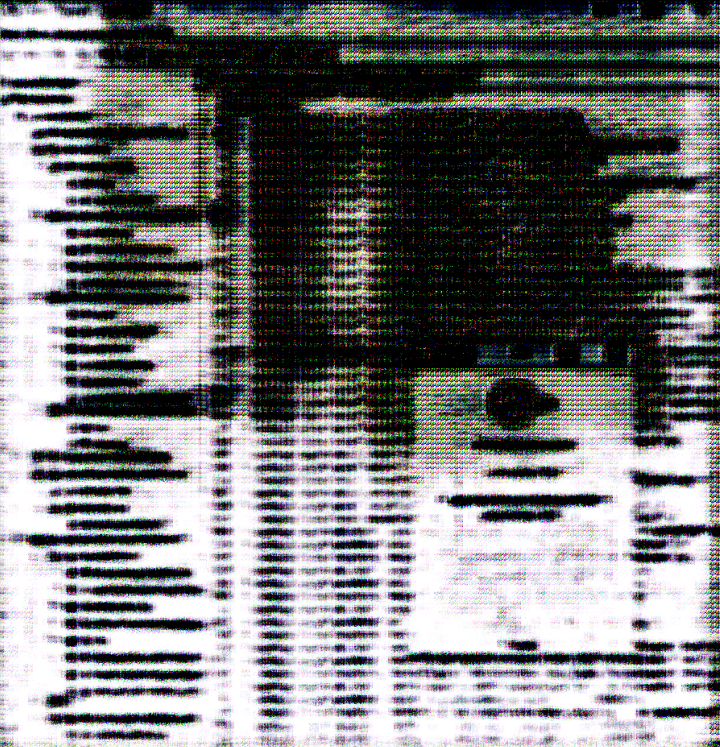
\includegraphics[width=0.6\textwidth]{bilder/image_relu_problems.png}
    \caption{Bildstörungen bei Verwendung der ReLU- und LeakyReLU-Aktivierungsfunktion als letzte Schicht}
    \label{fig:image_relu_problems}
\end{figure}

Während der Entwicklung stellte sich als wichtig heraus, dass die Convolutional-Schichten der Autoencoder über ein ausreichend großes Padding verfügen. Dieses Padding sorgt dafür, dass der Filter einer Convolutional-Schicht nicht an den Rändern der Eingabe beginnt, sondern über die Eingabe hinaus geht. Die Ränder und insbesondere die Ecken der Eingabe werden somit häufiger als Eingabe für die Filter verwendet. Ohne Padding würden beispielsweise die Ecken der Eingabe nur ein einziges Mal als Eingabe für die Filter verwendet, womit diese deutlich unterrepräsentiert wären. Damit ist ein Padding wichtig, um eine über das Bild hinweg gleichmäßig hohe Rekonstruktionsqualität zu erreichen. Insbesondere in der ersten Schicht der Autoencoder, in welcher die Eingabe und die Filter am größten sind, stellte sich die Verwendung eines Paddings als wichtig heraus. Dieses wurde in der Regel genauso groß wie der Filter gewählt. In den weiteren Schichten betrug die Größe des Paddings meist 1.

Darüber hinaus war es wichtig, dass die Aktivierungsfunktionen innerhalb des Decoder-Teils in etwa den Wertebereich [0,1] aufweisen. Es wurden Versuche durchgeführt, die ReLU- sowie die LeakyReLU-Funktion im Decoder-Teil des Autoencoders einzusetzen. Dies führte jedoch zu großflächigen Störungen, wie in Abb.~\ref{fig:image_relu_problems} dargestellt. Hier war zwar die grobe Bildeinteilung noch sichtbar, der Inhalt jedoch nicht mehr erkennbar.

Des Weiteren wurden Versuche unternommen, die Funktion \texttt{torch.BCELossWithLogits}\footnote{\url{https://pytorch.org/docs/stable/generated/torch.nn.BCEWithLogitsLoss.html}, letzter Zugriff: 13.12.2021} als Fehlerfunktion einzusetzen, die die binäre Kreuzentropie mit einer Sigmoid-Schicht verbindet und dadurch eine höhere numerische Stabilität erreicht. Die Ergebnisse waren jedoch schlechter als bei einer Verwendung der reinen binären Kreuzentropie. Dies könnte damit zusammenhängen, dass durch die zusätzliche Sigmoid-Schicht zwei Sigmoid-Funktionen nacheinander zum Einsatz kamen, da die letzte Schicht der Autoencoder ebenso die Sigmoid-Funktion beinhaltet. Dieser Zusammenhang kann in Zukunft genauer untersucht werden.

Daneben ist zu beachten, dass der Filter einer Convolutional-Schicht nicht deutlich kleiner ist, als das anschließend durchgeführte Pooling.
Hieraus resultierten Schachbrettmuster und eine schlechtere Bildqualität. Der Hintergrund für diese Beobachtung könnte sein, dass Pooling-Vorgänge nicht überlappend sind. Wenn der Filter der vorherigen Convolutional-Schicht nun sehr klein ist, werden Informationen über Bildbereiche hinweg, die größer sind als der Filter aber kleiner als die durch das Pooling zusammengefassten Bildbereiche, unter Umständen während der Faltung nicht erkannt und beim Pooling verworfen.


